
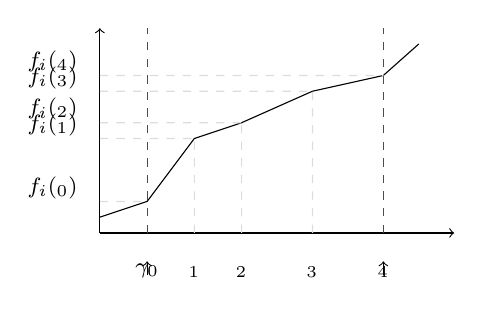
\begin{tikzpicture}
  [node distance=2cm,inner sep=0,xscale=0.3,yscale=0.2]
  
  \node (O) at (0,0) {};
  \node (A) at (2,2) {};
  \node (B) at (4,6) {};
  \node (C) at (6,7) {};
  \node (D) at (9,9) {};
  \node (E) at (12,10) {};
  \node (F) at (13.5,12) {};
  
  \node[label={[shift={(0,-0.6)}]\footnotesize $\gamma_0$}] (ga0) at (2,0) {};
  \node[label={[shift={(0,-0.6)}]\footnotesize $\ga_1$}] (ga1) at (4,0) {};
  \node[label={[shift={(0,-0.6)}]\footnotesize $\ga_2$}] (ga2) at (6,0) {};
  \node[label={[shift={(0,-0.6)}]\footnotesize $\ga_3$}] (ga3) at (9,0) {};
  \node[label={[shift={(0,-0.6)}]\footnotesize $\ga_4$}] (ga4) at (12,0) {};
  \node[label={[shift={(-0.6,0)}]\footnotesize $f_i(\ga_0)$}] (f0) at (0,2) {};
  \node[label={[shift={(-0.6,0)}]\footnotesize $f_i(\ga_1)$}] (f1) at (0,6) {};
  \node[label={[shift={(-0.6,0)}]\footnotesize $f_i(\ga_2)$}] (f2) at (0,7) {};
  \node[label={[shift={(-0.6,0)}]\footnotesize $f_i(\ga_3)$}] (f3) at (0,9) {};
  \node[label={[shift={(-0.6,0)}]\footnotesize $f_i(\ga_4)$}] (f4) at (0,10) {};
  
  
  \draw[->] (O.center) -- (0,13);
  \draw[->] (O.center) -- (15,0);
  \draw (0,1) -- (A.center) -- (B.center) -- (C.center) -- (D.center) -- (E.center) -- (F.center);
  
  \draw[dashed,red] (2,0) -- (2,13);
  \draw[dashed,red] (12,0) -- (12,13);
  
  \draw[dashed,Gainsboro] (4,0) -- (B.center);
  \draw[dashed,Gainsboro] (6,0) -- (C.center);
  \draw[dashed,Gainsboro] (9,0) -- (D.center);
  
  \draw[dashed,Gainsboro] (0,2) -- (A.center);
  \draw[dashed,Gainsboro] (0,6) -- (B.center);
  \draw[dashed,Gainsboro] (0,7) -- (C.center);
  \draw[dashed,Gainsboro] (0,9) -- (D.center);
  \draw[dashed,Gainsboro] (0,10) -- (E.center);
  

  \draw[<-]  (2,-1.8) -- (2,-2.7) node[label={[shift={(0,-0.4)}]\footnotesize $\bmin$}]{};
  \draw[<-]  (12,-1.8) -- (12,-2.7) node[label={[shift={(0,-0.4)}]\footnotesize $\bmax$}]{};
\end{tikzpicture}
